%-------------------------------------------------------------------------------
%                                PREAMBLE
%-------------------------------------------------------------------------------
\documentclass[usenames,dvipsnames,svgnames,10pt,aspectratio=169]{beamer}
%
\usefonttheme{professionalfonts}
% This theme uses TIKZ: compile twice with PDFLaTeX or LuaLaTeX.
%
%  Options:
%  - [clean]:    clean slides, i.e. logos and footbar are removed
%  - [kth]:      footbar style inspierd to the official KTH template
%  - [nicewave]: a different style of wave is used (not approved by FLOW)
%
\usetheme[clean]{flow}

\usepackage{tikz}
\usetikzlibrary{arrows}
\usetikzlibrary{shapes.geometric, math, positioning, calc, patterns, angles, quotes}
\usetikzlibrary{patterns.meta,decorations.pathmorphing}

\newcommand{\semaphore}[3]{% #1: color of circle,
                           % #2: color of semicircle
                           % #3: angle of semicircle 
  \tikz[node distance=0mm,baseline]
       {
         \node (s1) [circle, fill=#1, minimum size=6mm] {};
         \node      [semicircle, fill=#2, 
           inner sep=0pt, outer sep=0pt, minimum size=3mm,
           anchor=south,
           at={(s1.center)}, rotate=#3] {};
       }
}

\usepackage[]{circuitikz}

\usepackage{pgfplots}
\usepgfplotslibrary{polar}

\usepackage{hyperref,graphicx,lmodern}
\usepackage[utf8]{inputenc}
\usepackage{media9}
\usepackage{xcolor}
\usepackage{stmaryrd}
\usepackage{nicefrac}
\usepackage{multimedia}
\usepackage{multicol}
\usepackage{upgreek}
\usepackage[]{bm}
\usepackage[]{url}
\usepackage[]{animate}
\usepackage{amsmath}

\usepackage[most]{tcolorbox}

\graphicspath{{imgs/}}
\setbeamertemplate{blocks}[rounded][shadow=true]

\DeclareMathOperator*{\maximize}{maximize~}

%-------------------------------------------------------------------------------
%                                TITLE PAGE
%-------------------------------------------------------------------------------
\title[Nonlinear physics] % Short title used in footline
{
	Strongly nonlinear oscillators \\
  and relaxation oscillations
}

\author[J.-Ch.~Loiseau] % Presenting author in short form used in footline
{
	\underline{Jean-Christophe Loiseau}
}
% - Give the names in the same order as the appear in the paper.
% - Underline the presenting author.

\institute[unused]
{
	\url{jean-christophe.loiseau@ensam.eu} \\
	Laboratoire DynFluid \\
	Arts et M\'etiers, France.
}
% Keep it simple, no one is interested in your street address.

% University logo(s)
\logot{
\includegraphics[width=.128\paperwidth]{DynFluid_logo}}  % Top logo
\logob{
\includegraphics[width=0.128\paperwidth]{ENSAM_logo}} % Bottom logo
% \logoc[{\includegraphics[width=.128\paperwidth]{limsi}}]{\includegraphics[width=.128\paperwidth]{limsi}} % Corner logo
%
% Cover image: \cvrimg{x position}{y position}{cover image}
\cvrimg{.77}{.8}{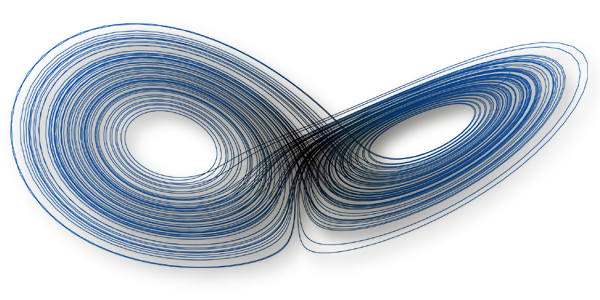
\includegraphics[width=.4\paperwidth]{cover.png}}

\date[unused]{Physique non-lin\'eaire -- 2019-2020}

\begin{document}

\titleframe	% Print the title as the first slide

%-------------------------------------------------------------------------------
%                           PRESENTATION SLIDES
%-------------------------------------------------------------------------------

\begin{frame}[t, c]{Strongly nonlinear oscillators}{Example : van der Pol oscillator}

  \begin{minipage}{.68\textwidth}
    \[
    \tcboxmath[colframe=beamer@kthblue, colback=white]{
      \textbf{van der Pol osc.\ :} \quad \ddot{x} + \mu \left( x^2 - 1 \right) \dot{x} + x = 0
    }
    \]

    \bigskip

    For small values of $\mu$, the dynamics are those of a weakly nonlinear oscillator.
    But what if $\mu$ is much larger than unity?
    Can we say anything meaningful about them from a theoretical point of view?

  \end{minipage}%
  \hfill
  \begin{minipage}{.28\textwidth}
    \centering
    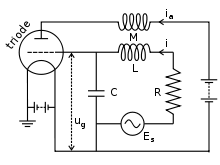
\includegraphics[width=\textwidth]{van_der_pol}
  \end{minipage}
\end{frame}





\begin{frame}[t, c]{Strongly nonlinear oscillators}{Relaxation oscillations}
  
  \centering
  \begin{tikzpicture}[>=stealth]
    \draw[->, thick] (-1, 0) -- (7, 0) node[below] {$t$};
    \draw[->, thick] (0, -1.25) -- (0, 1.25) node[left] {$x$};
    
    \draw[gray, thick] plot file{traj_1.txt};
  \end{tikzpicture}
\end{frame}

\begin{frame}[t, c]{Strongly nonlinear oscillators}{Relaxation oscillations}

  \centering
  \begin{tikzpicture}[>=stealth]
    \draw[->, thick] (-1, 0) -- (7, 0) node[below] {$t$};
    \draw[->, thick] (0, -1.25) -- (0, 1.25) node[left] {$x$};
    
    \draw[gray, thick] plot file{traj_2.txt};
  \end{tikzpicture}
  
 \end{frame}

\begin{frame}[t, c]{Strongly nonlinear oscillators}{Relaxation oscillations}
  \centering
  \begin{tikzpicture}[>=stealth]
    \draw[->, thick] (-1, 0) -- (7, 0) node[below] {$t$};
    \draw[->, thick] (0, -1.25) -- (0, 1.25) node[left] {$x$};
    
    \draw[gray, thick] plot file{traj_3.txt};
  \end{tikzpicture}
\end{frame}





\begin{frame}[t, c]{Strongly nonlinear oscillators}{Why does it matters?}
  \centering
\end{frame}





\begin{frame}[t, c]{Strongly nonlinear oscillators}{How to study these relaxation oscillations?}
  \begin{overprint}
    \onslide<1>
    \[
    \ddot{x} + \mu \left( x^2 - 1 \right) \dot{x} + x = 0
    \]
    
    \onslide<2>
    \[
    \dfrac{d}{dt} \underbrace{\left(\dot{x} + \mu \left( \dfrac{x^3}{3} - x \right) \right)}_{w} + x = 0
    \]
    
    \onslide<3>
    \[
    \begin{aligned}
      \dot{w} & = - x \\
      \dot{x} & = w + \mu \left( x - \dfrac{x^3}{3} \right)
    \end{aligned}
    \]

    \onslide<4>
    \[
    \begin{aligned}
      \dfrac{\dot{w}}{\mu} & = - \dfrac{x}{\mu} \\
      \dfrac{\dot{x}}{\mu} & = \dfrac{w}{\mu} + x - \dfrac{x^3}{3}
    \end{aligned}
    \]

    \onslide<5>
    \[
    \begin{aligned}
      \dot{y} & = - \epsilon x \\
      \epsilon \dot{x} & = y + x - \dfrac{x^3}{3}
    \end{aligned}
    \]
    
  \end{overprint}
\end{frame}





\begin{frame}[t, c]{Strongly nonlinear oscillators}{Boundary layers in time}
  \centering
  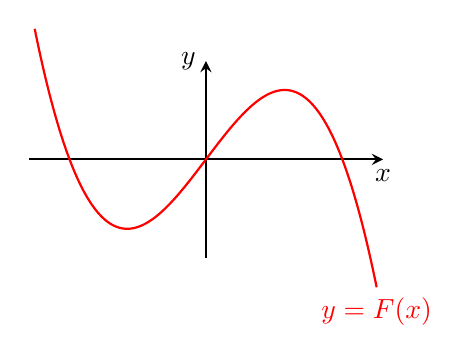
\begin{tikzpicture}[>=stealth]
    \draw[->, thick] (-2.25, 0) -- (2.25, 0) node[below] {$x$};
    \draw[->, thick] (0, -1.25) -- (0, 1.25) node[left] {$y$};

    \draw[red, thick, variable=\x, domain=-2.175:2.175, smooth, samples=512] plot (\x, {(\x - \x^3/3)/0.7564466}) node[below] {$y = F(x)$};    
    \draw[gray, thick] plot file{phase_portrait_3.txt};

  \end{tikzpicture}
\end{frame}

\begin{frame}[t, c]{Strongly nonlinear oscillators}{Boundary layers in time}
  \centering
  \begin{tikzpicture}[>=stealth]
    \draw[->, thick] (-1, 0) -- (7, 0) node[below] {$t$};
    \draw[->, thick] (0, -1.25) -- (0, 1.25) node[left] {$x$};

    \draw[-, thick] (1.55, -1.2) -- (2.15, -1.2) node[below left] {$\mathcal{O}(\mu)$};
    \draw[-, thick] (1.55, -1.15) -- (1.55, -1.25) {};
    \draw[-, thick] (2.15, -1.15) -- (2.15, -1.25) {};

    \draw[-, thick] (2.15, 1.2) -- (2.25, 1.2) node[above] {$\mathcal{O}(\mu^{-1})$};
    \draw[-, thick] (2.15, 1.15) -- (2.15, 1.25) node[] {};
    \draw[-, thick] (2.25, 1.15) -- (2.25, 1.25) node[] {};

    \draw[gray, thick] plot file{traj_3.txt};
  \end{tikzpicture}
\end{frame}

\begin{frame}[t, c]{Strongly nonlinear oscillators}{The slow time-scale}
  \begin{minipage}{.58\textwidth}
    \begin{overprint}
      \onslide<1>
      On the slow branches, we have $y \simeq F(x)$, hence
      %
      \[
      \dfrac{dy}{dt} \simeq F'(x) \dfrac{dx}{dt} = \left( x^2 - 1 \right) \dfrac{dx}{dt}.
      \]
      %
      Using the equations of the system, we can find
      %
      \[
      dt \simeq -\dfrac{\mu \left( x^2 - 1 \right)}{x} dx
      \]

      \onslide<2>
      From symmetry arguments, we can then show that the period of oscillation is
      %
      \[
      T \simeq -2\mu \int_{2}^{1} \dfrac{x^2 - 1}{x} dx = \mu \left( 3 - 2 \ln 2 \right).
      \]
      %
      which is $\mathcal{O}(\mu)$ as expected.

    \end{overprint}
  \end{minipage}%
  \hfill
  \begin{minipage}{.38\textwidth}
    \centering
    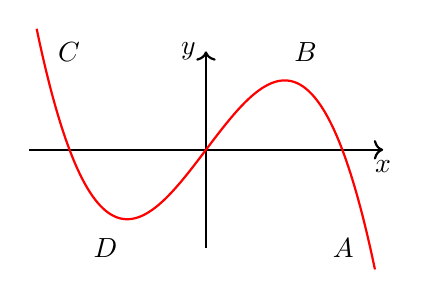
\begin{tikzpicture}
      \draw[->, thick] (-2.25, 0) -- (2.25, 0) node[below] {$x$};
      \draw[->, thick] (0, -1.25) -- (0, 1.25) node[left] {$y$};
      
      \draw[red, thick, variable=\x, domain=-2.15:2.15, smooth, samples=512] plot (\x, {(\x - \x^3/3)/0.7564466}) node[] {};    
      \draw[gray, thick] plot file{phase_portrait_3.txt};

      \node[below left] at (2, -1) {$A$};
      \node[above right] at (1, 1) {$B$};
      \node[above right] at (-2, 1) {$C$};
      \node[below left] at (-1, -1) {$D$};
      
    \end{tikzpicture}
  \end{minipage}

\end{frame}





\begin{frame}[t, c]{Boundary layer in time}{A linear example}
  \begin{minipage}{.68\textwidth}
    \begin{overprint}
      \onslide<1>
      \[
      mL^2 \ddot{\theta} + b \dot{\theta} + mgL \sin(\theta) = 0
      \]

      \onslide<2>
      \[
      \dfrac{L}{g \tau^2} \ddot{\theta} + \dfrac{b}{mgL \tau} \dot{\theta} + \sin(\theta) = 0
      \]

      \onslide<3>
      \[
       \dfrac{m^2 L^3 g}{b^2} \ddot{\theta} + \dot{\theta} + \sin(\theta) = 0
       \]

       \onslide<4>
       \[
       \epsilon \ddot{\theta} + \dot{\theta} + \sin(\theta) = 0
       \]

       \onslide<5>
       \[
       \begin{aligned}
         & \epsilon \ddot{\theta} + \dot{\theta} + \theta = 0 \\
         \text{with} \quad & \theta_0 = 0 \quad \text{and} \quad \dot{\theta}_0 = 1.
       \end{aligned}
       \]

    \end{overprint}
  \end{minipage}%
  \hfill
  \begin{minipage}{.28\textwidth}
  \end{minipage}
\end{frame}




\begin{frame}[t, c]{Boundary layer in time}{A linear example}
  \centering
  \begin{tikzpicture}[>=stealth]
    \draw[->, thick] (-1, 0) -- (10, 0) node[below] {$t$};
    \draw[->, thick] (0, -0.5) -- (0, 2) node[left] {$x(t)$};
  \end{tikzpicture}
\end{frame}




\begin{frame}[t, c]{Boundary layer in time}{A linear example}
  Let us consider the outer layer defined by $t \gg 1$.
  Using regular perturbation theory, i.e. expanding the solution as
  %
  \[
  x(t, \epsilon) = x_0(t) + \epsilon x_1(t) + \cdots
  \]
  %
  leads to
  %
  \[
  \begin{aligned}
    \mathcal{O}(1) : \quad & \dot{x}_0 + x_0 = 0 \\
    \mathcal{O}(\epsilon) : \quad & \dot{x}_1 + x_1 = - \ddot{x}_0
  \end{aligned}
  \]
  %
  Note that we do not consider initial conditions since they would need to be applied inside the initial layer.
\end{frame}


\begin{frame}[t, c]{Boundary layer in time}{A linear example}
  \[
  \tcboxmath[colframe=beamer@kthblue, colback=white]{
    \textbf{Outer solution :} \quad x_{\text{out}}(t) = \epsilon A e^{-t} + \cdots
  }
  \]
\end{frame}



\end{document}
